\documentclass[pdflatex,compress,mathserif]{beamer}

%\usetheme[dark,framenumber,totalframenumber]{ElektroITK}
\usetheme[darktitle,framenumber,totalframenumber]{ElektroITK}

\usepackage[utf8]{inputenc}
\usepackage[T1]{fontenc}
\usepackage{lmodern}
\usepackage[english]{babel}
\usepackage{amsmath}
\usepackage{amsfonts}
\usepackage{amssymb}
\usepackage{graphicx}
\usepackage{multicol}
\usepackage{lipsum}
\usepackage{framed}
\usepackage{minted}

\definecolor{LightGray}{gray}{0.95}

\usefonttheme[onlymath]{serif}

\newcommand*{\Scale}[2][4]{\scalebox{#1}{$#2$}}%

\setbeamertemplate{caption}[numbered]

\title{Digital Signal Processing}
\subtitle{Infinite Impulse Response}

\author{Mifta Nur Farid}

\begin{document}

\maketitle

\begin{frame}{Infinite Impulse Response Filter\\Format}
    \begin{itemize}
        \item An IIR filter is described using the difference equation
        \begin{figure}
            \centering
            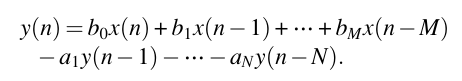
\includegraphics[width=0.8\linewidth]{./img/img01.png}
        \end{figure}
        \item the IIR filter transfer function as
        \begin{figure}
            \centering
            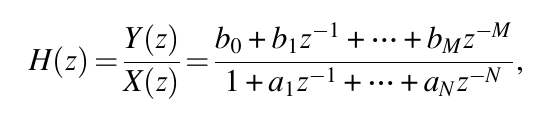
\includegraphics[width=0.7\linewidth]{./img/img02.png}
        \end{figure}
        where $b_i$ and $a_i$ are the $(M+1)$ numerator and $N$ denominator coefficients, respectively.
    \end{itemize}
\end{frame}

\begin{frame}{Bilinear Transformation Design\\Method}
    \begin{itemize}
        \item General procedure for IIR filter design using BLT:
        \begin{figure}
            \centering
            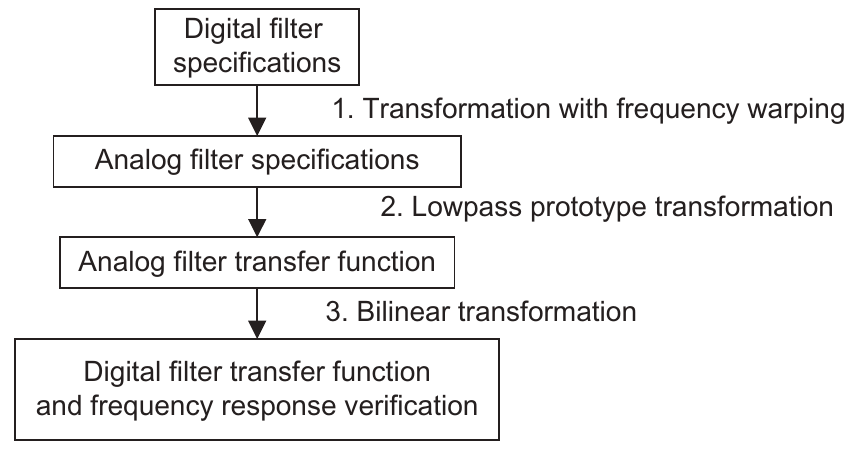
\includegraphics[width=\linewidth]{./img/img03.png}
        \end{figure}
    \end{itemize}
\end{frame}

\begin{frame}{Bilinear Transformation Design\\Method}
    \begin{enumerate}
        \item Transformation with frequency warping
        \begin{itemize}
            \item For the lowpass filter and the highpass filter:
            \begin{figure}
                \centering
                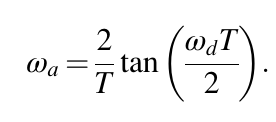
\includegraphics[width=0.4\linewidth]{./img/img04.png}
            \end{figure}
            \item For the bandpass filter and the bandstop filter:
            \begin{figure}
                \centering
                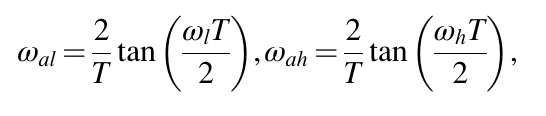
\includegraphics[width=0.7\linewidth]{./img/img05.png}
                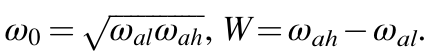
\includegraphics[width=0.6\linewidth]{./img/img06.png}
            \end{figure}
        \end{itemize}
    \end{enumerate}
\end{frame}

\begin{frame}{Bilinear Transformation Design\\Method}
    \begin{enumerate}
        \setcounter{enumi}{1}
        \item Lowpass prototype transformation
        \begin{figure}
            \centering
            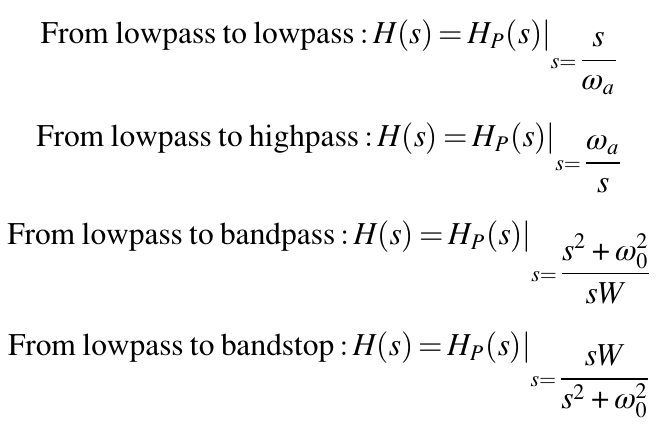
\includegraphics[width=0.9\linewidth]{./img/img07.png}
        \end{figure}
    \end{enumerate}
\end{frame}

\begin{frame}{Bilinear Transformation Design\\Method}
    \begin{enumerate}
        \setcounter{enumi}{2}
        \item Bilinear transformation
        \begin{figure}
            \centering
            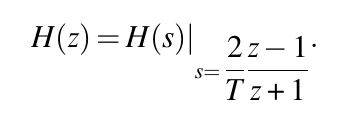
\includegraphics[width=0.5\linewidth]{./img/img08.png}
        \end{figure}
    \end{enumerate}
\end{frame}

\begin{frame}{Example}
    \begin{figure}
        \centering
        
\includegraphics[width=\linewidth]{./img/img09a.png}
        
\includegraphics[width=\linewidth]{./img/img09b.png}
    \end{figure}
\end{frame}

\begin{frame}{Example}
    \begin{figure}
        \centering
        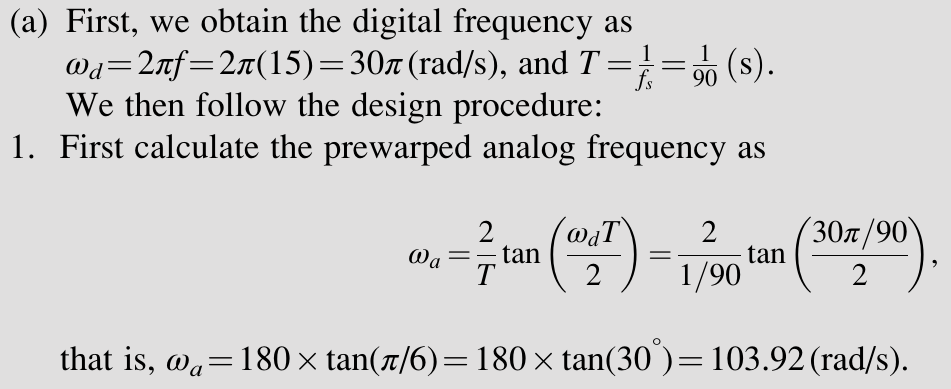
\includegraphics[width=\linewidth]{./img/img10.png}
    \end{figure}
\end{frame}

\begin{frame}{Example}
    \begin{figure}
        \centering
        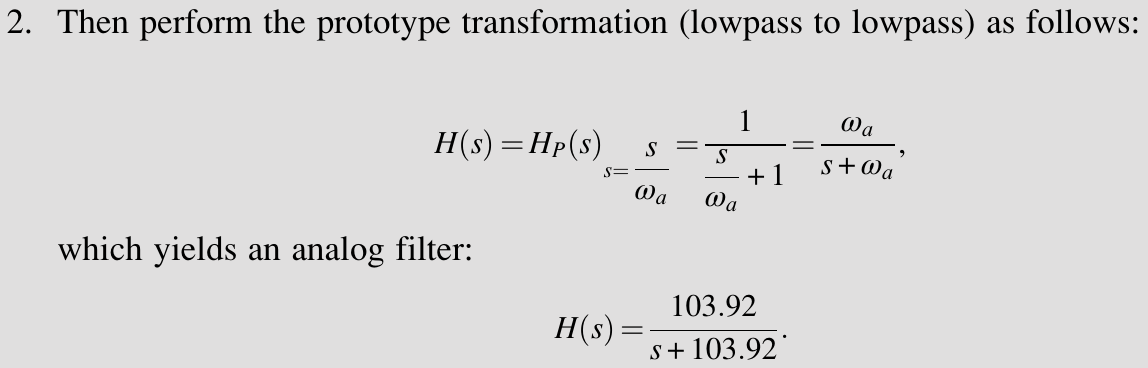
\includegraphics[width=\linewidth]{./img/img11.png}
    \end{figure}
\end{frame}

\begin{frame}{Example}
    \begin{figure}
        \centering
        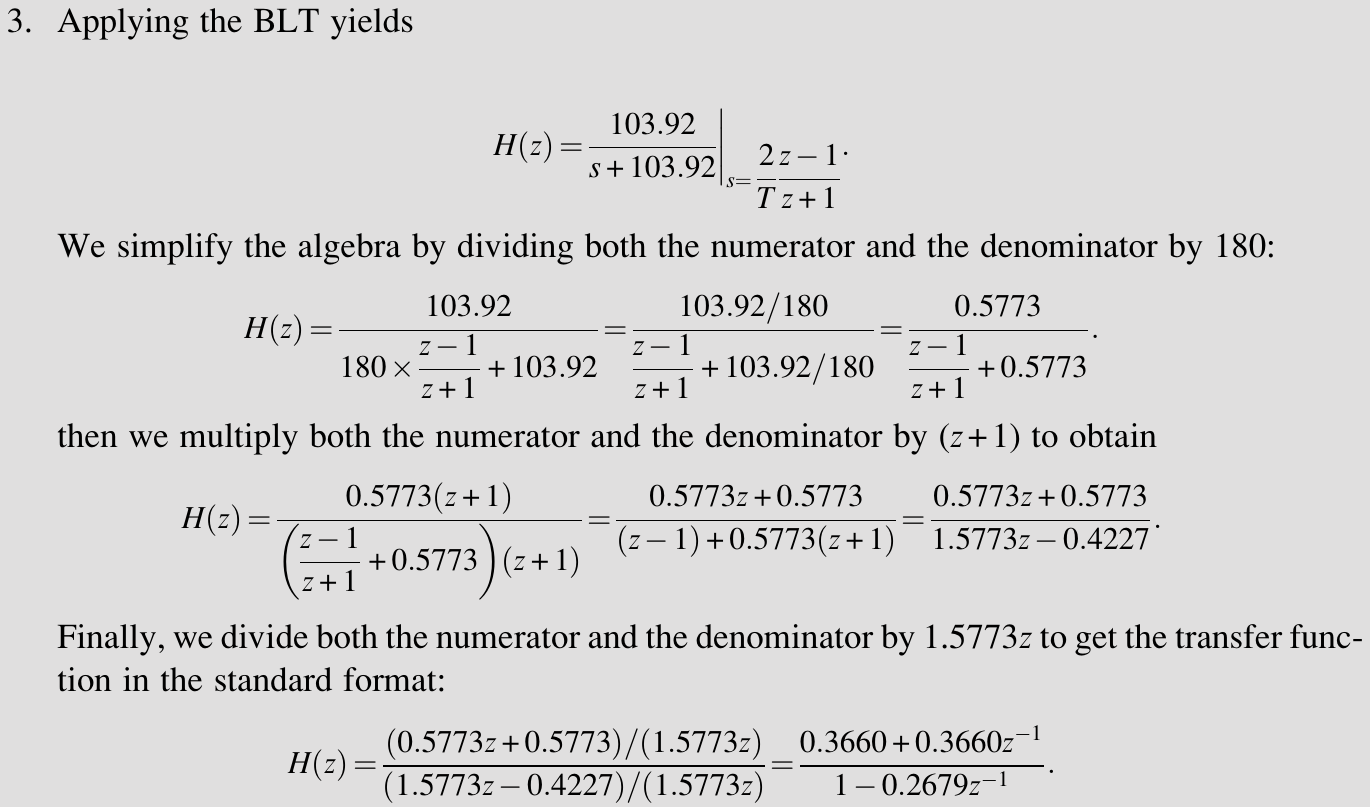
\includegraphics[width=\linewidth]{./img/img12.png}
    \end{figure}
\end{frame}

\begin{frame}{Digital Butterworth and Chebyshev\\Filter Designs}
    \begin{figure}
        \centering
        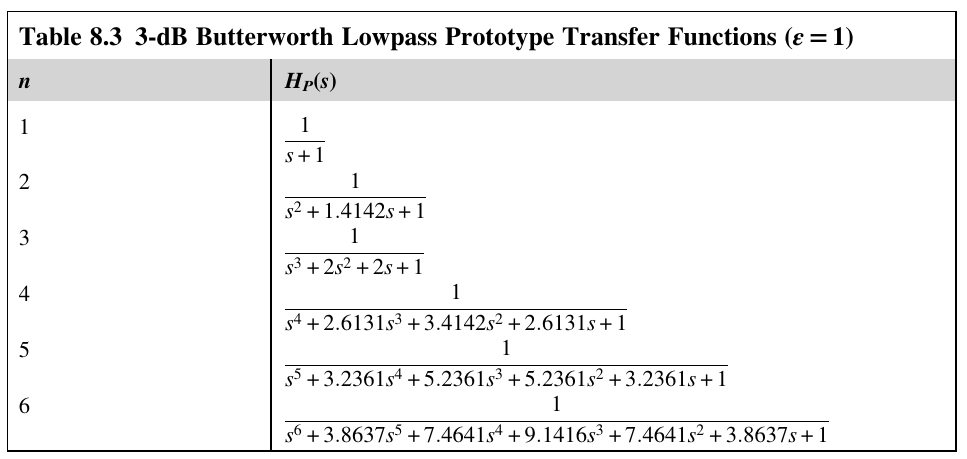
\includegraphics[width=\linewidth]{./img/img13.png}
    \end{figure}
\end{frame}

\begin{frame}{Digital Butterworth and Chebyshev\\Filter Designs}
    \begin{figure}
        \centering
        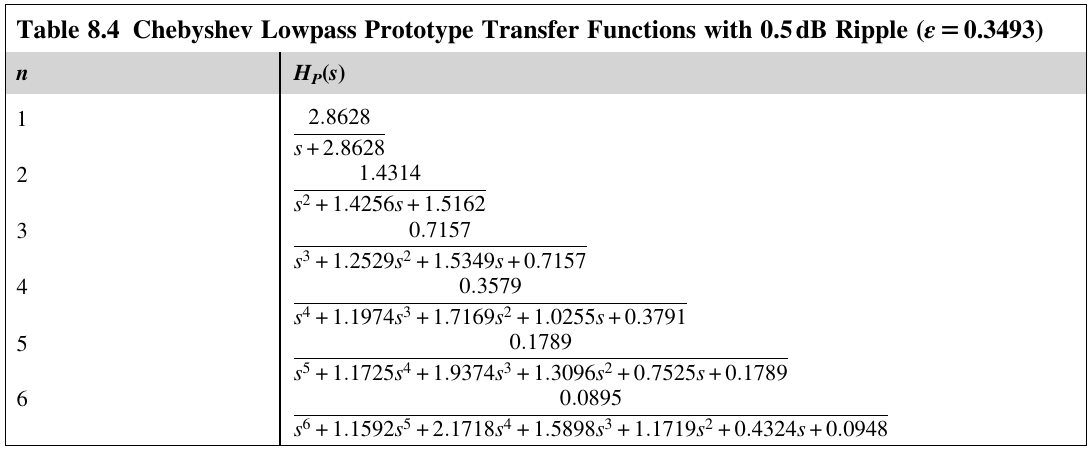
\includegraphics[width=\linewidth]{./img/img14.png}
    \end{figure}
\end{frame}

\begin{frame}{Digital Butterworth and Chebyshev\\Filter Designs}
    \begin{figure}
        \centering
        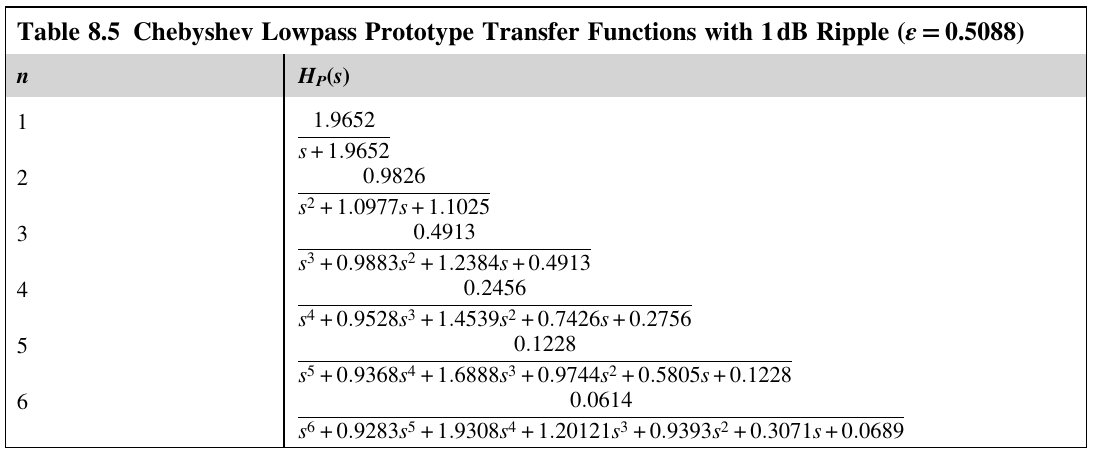
\includegraphics[width=\linewidth]{./img/img15.png}
    \end{figure}
\end{frame}

\begin{frame}{Digital Butterworth and Chebyshev\\Filter Designs}
    \begin{figure}
        \centering
        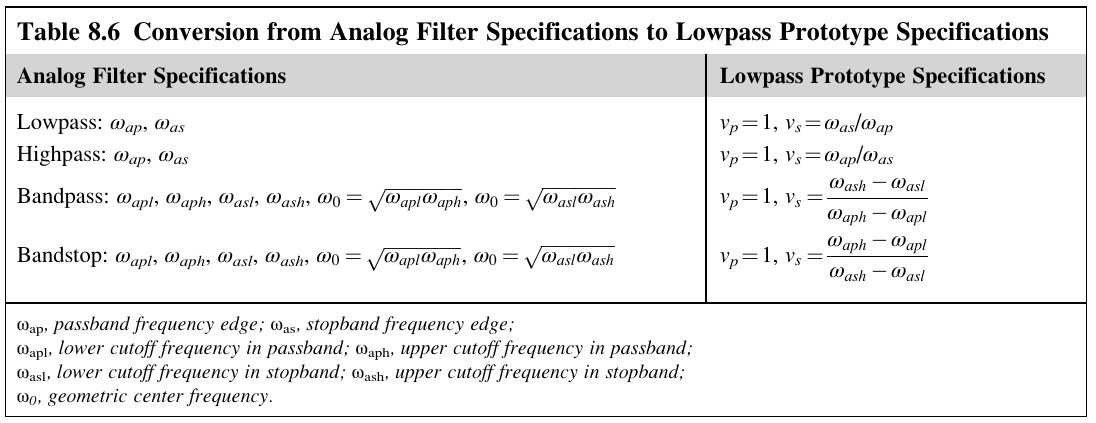
\includegraphics[width=\linewidth]{./img/img16.png}
    \end{figure}
\end{frame}

\begin{frame}{Example}
    \begin{figure}
        \centering
        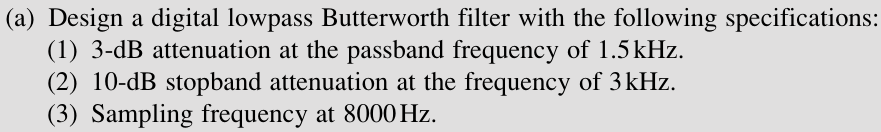
\includegraphics[width=\linewidth]{./img/img17.png}
    \end{figure}
\end{frame}

\begin{frame}{Example}
    \begin{figure}
        \centering
        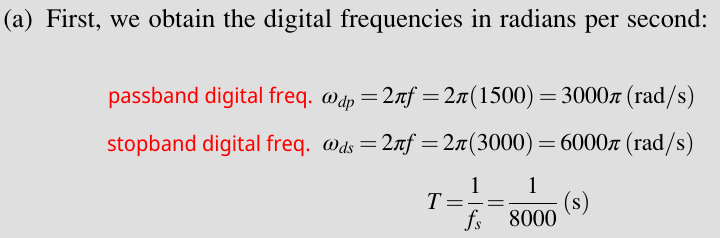
\includegraphics[width=\linewidth]{./img/img18.png}
    \end{figure}
\end{frame}

\begin{frame}{Example}
    \begin{figure}
        \centering
        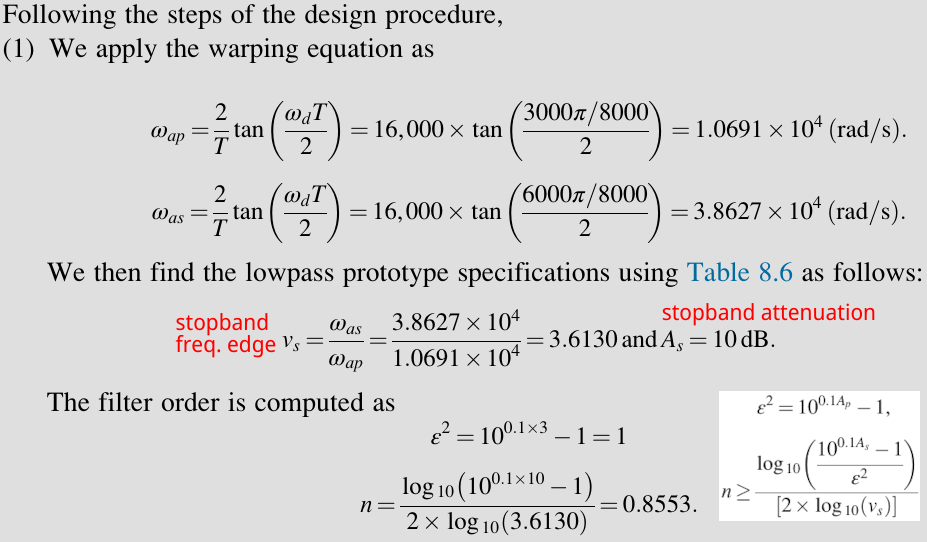
\includegraphics[width=\linewidth]{./img/img19.png}
    \end{figure}
\end{frame}

\begin{frame}{Example}
    \begin{figure}
        \centering
        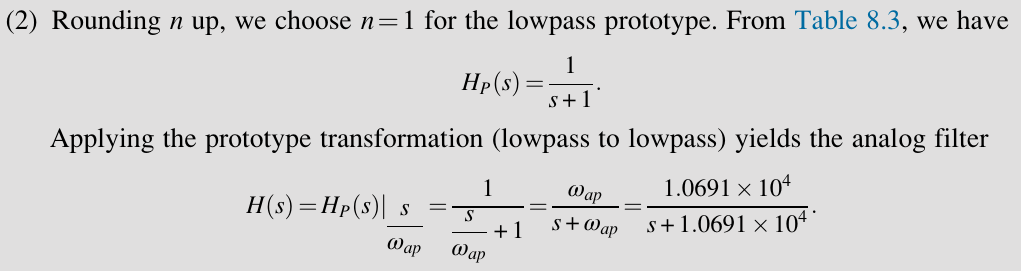
\includegraphics[width=\linewidth]{./img/img20.png}
        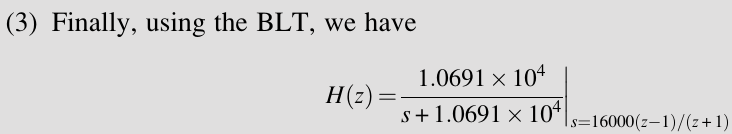
\includegraphics[width=\linewidth]{./img/img21.png}
    \end{figure}
\end{frame}

\begin{frame}{Example}
    \begin{figure}
        \centering
        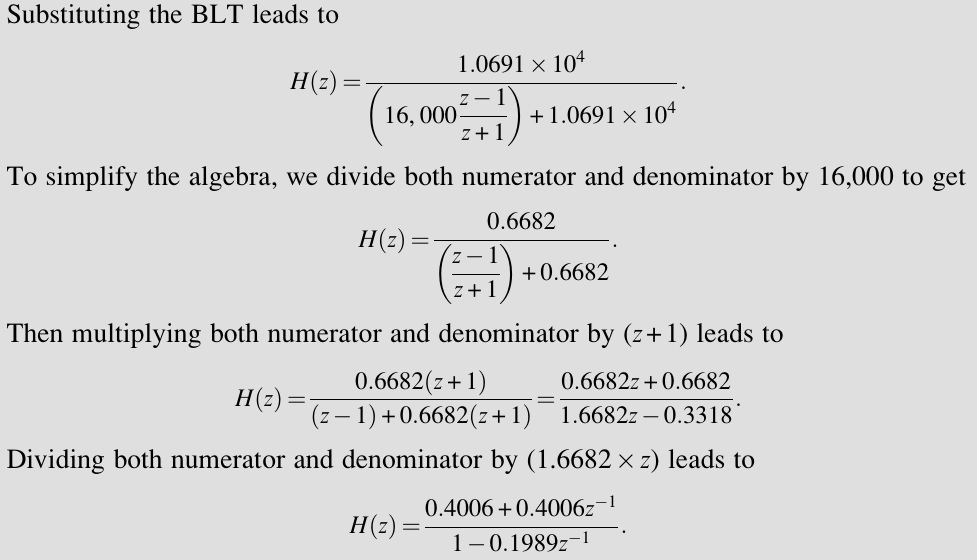
\includegraphics[width=\linewidth]{./img/img22.png}
    \end{figure}
\end{frame}

\begin{frame}{Example}
    \begin{figure}
        \centering
        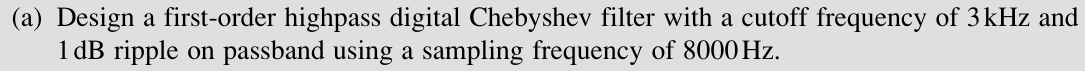
\includegraphics[width=\linewidth]{./img/img23.png}
    \end{figure}
\end{frame}

\end{document}